\chapter{Performance and Validation}

\section{Test Setup}
To ensure both precise laboratory validation and real-world functional verification, the device was subjected to four distinct testing configurations:

\begin{description}
    \item[Setup 1: Wall Adapter (Unloaded)] A standard commercial USB Type-C wall adapter was connected to the WattMate input port, with the output port left unconnected. This setup was used to verify the initial boot sequence without load-induced voltage drops.
    
    \item[Setup 2: Wall Adapter to Smartphone] A wall adapter was connected to the input, and a commercial smartphone was connected to the output port. This configuration represents the primary real-world use case of the device, allowing for dynamic load testing as the phone's internal battery management system negotiates power.
    
    \item[Setup 3: DC Power Supply (Unloaded)] A precision laboratory DC power supply was injected into the input port, with the output floating. This setup provided highly regulated, noise-free power and allowed for manual, precise adjustments of the input voltage to test the system's operational boundaries.
    
    \item[Setup 4: DC Power Supply to Resistive Load] The laboratory DC power supply drove the input, while a resistive load was connected to the output. This configuration allowed for strict, controlled current draws to test the thermal dissipation of the PCB and the linearity of the analog current sensing circuit.
\end{description}



\begin{figure}[H]
\centering

% ===================== SETUP 1 =====================
\begin{tikzpicture}[
    block/.style={draw, rounded corners, minimum width=3cm, minimum height=0.9cm, align=center},
    arrow/.style={->, thick}
]
\node[block] (in) {Wall Adapter\\(USB-C)};
\node[block, right=2.8cm of in] (dev) {WattMate};
\node[block, right=2.8cm of dev] (out) {Unloaded\\(Open Circuit)};

\draw[arrow] (in) -- (dev);
\draw[arrow] (dev) -- (out);

\node at ($(in)!0.5!(out) + (0,-1.2)$) {Setup 1: Unloaded Wall Adapter};

\end{tikzpicture}

\vspace{0.6cm}

% ===================== SETUP 2 =====================
\begin{tikzpicture}[
    block/.style={draw, rounded corners, minimum width=3cm, minimum height=0.9cm, align=center},
    arrow/.style={->, thick}
]
\node[block] (in) {Wall Adapter\\(USB-C)};
\node[block, right=2.8cm of in] (dev) {WattMate};
\node[block, right=2.8cm of dev] (out) {Smartphone\\Load};

\draw[arrow] (in) -- (dev);
\draw[arrow] (dev) -- (out);

\node at ($(in)!0.5!(out) + (0,-1.2)$) {Setup 2: Smartphone Load};

\end{tikzpicture}

\vspace{0.6cm}

% ===================== SETUP 3 =====================
\begin{tikzpicture}[
    block/.style={draw, rounded corners, minimum width=3cm, minimum height=0.9cm, align=center},
    arrow/.style={->, thick}
]
\node[block] (in) {Laboratory\\DC Power Supply};
\node[block, right=2.8cm of in] (dev) {WattMate};
\node[block, right=2.8cm of dev] (out) {Unloaded\\(Open Circuit)};

\draw[arrow] (in) -- (dev);
\draw[arrow] (dev) -- (out);

\node at ($(in)!0.5!(out) + (0,-1.2)$) {Setup 3: DC Supply Unloaded};

\end{tikzpicture}

\vspace{0.6cm}

% ===================== SETUP 4 =====================
\begin{tikzpicture}[
    block/.style={draw, rounded corners, minimum width=3cm, minimum height=0.9cm, align=center},
    arrow/.style={->, thick}
]
\node[block] (in) {Laboratory\\DC Power Supply};
\node[block, right=2.8cm of in] (dev) {WattMate};
\node[block, right=2.8cm of dev] (out) {Resistive Load};

\draw[arrow] (in) -- (dev);
\draw[arrow] (dev) -- (out);

\node at ($(in)!0.5!(out) + (0,-1.2)$) {Setup 4: Resistive Load Test};

\end{tikzpicture}

\caption{Test setups used for validation of the WattMate system under different input sources and load conditions.}
\label{fig:wattmate_setups}
\end{figure}



\section{Test Results}

\subsection{Initial Working Verification (\SI{5}{\volt})}
The initial functional verification was performed using both Setup 1 and Setup 3, providing a standard \SI{5}{\volt} VBUS input. In both scenarios, the MAX77597 step-down converter successfully activated, providing a stable \SI{3.260}{\volt} logic supply. The MCU successfully completed its boot sequence, initialized the $I^2C$ bus and the BLE communication, allowing external connection through the mobile application. However, under specific operating conditions, the OLED display failed to initialize. This behavior, alongside the deviations observed on the \SI{3.3}{\volt} logic rail, is discussed in detail in Section~\ref{problems}.

\subsection{Input DC Voltage Sweep (\SI{4}{\volt} to \SI{30}{\volt})}
To validate the high-voltage resilience of the system and the wide-input capabilities of the DC-DC converter, an input voltage sweep was performed using Setup 3. The DC power supply was slowly ramped from \SI{4}{\volt} up to a maximum over-voltage state of \SI{30}{\volt}. 
\par
Throughout the entire sweep, the \SI{3.3}{\volt} rail remained perfectly stable. Furthermore, the average voltage readings reported by the PAC1951 sensor via the MCU precisely matched the laboratory equipment's output, confirming that the sensing stage was implemented and initialized correctly. However, the recorded data exhibited a superimposed noise higher than expected, resulting in a flactuating reading.

\subsection{High-Current Load Testing (Up to \SI{3}{\ampere})}
Current sensing accuracy and thermal stability were validated using Setup 4. By adjusting the resistive load, the current drawn through the VBUS line was steadily increased in increments up to \SI{3}{\ampere}, reaching the limit of the DC power supply available in the laboratory. 
\par
The physical VBUS polygon pours and via arrays easily handled the current without significant thermal gradients. The current measurements demonstrated good linearity from \SI{100}{\milli\ampere} up to \SI{3}{\ampere}. AS for the voltage reading, the recorded data exhibited a superimposed noise higher than expected, resulting in a flactuating reading.

\subsection{State of Charge (SoC) Estimation}
The pseudo-real State of Charge (SoC) estimation was validated using Setup 2 by charging a smartphone from a depleted state. To validate the implemented algorithm and the charging cycle information management, the end-of-cycle energy threshold was temporarily reduced from its nominal value. This modification allowed multiple charging cycles to be completed in a shorter time, enabling repetitive testing without waiting for a full smartphone charge and subsequent discharge.

The system successfully tracked the passing energy throughout the entire cycle, with the OLED display accurately reflecting the real-time state of charge as the smartphone transitioned from charging to discharging cycles.

% Optional: Add a figure here if you have a plot of the voltage sweep or SoC curve!
% \begin{figure}[H]
%     \centering
%     \includegraphics[width=0.7\textwidth]{figures/soc_curve.png}
%     \caption{Measured State of Charge (SoC) estimation over time during the smartphone charging test (Setup 2).}
%     \label{fig:soc_test}
% \end{figure}

\section{Problems and Troubleshooting}\label{problems}

While the overall architecture performed as expected, several issues were identified during the hardware bring-up and validation phases:

\subsection{Measurement Noise}

During validation testing, the voltage, current, and temperature measurements exhibited a higher noise level than initially expected. Investigation revealed that the primary source of the issue was excessive ripple on the \SI{3.3}{\volt} power supply rail. Although the DC-DC converter was designed to operate at a switching frequency of \SI{1.7}{\mega\hertz}, its power-saving skip mode had been enabled. Under the relatively low load conditions of the system, the regulator automatically reduced its switching activity to improve efficiency and minimize switching losses. As a consequence, the output ripple became strongly non-stationary, exhibiting a dynamically varying periodic behavior.

In particular, the ripple frequency was observed to fluctuate between approximately \SI{350}{\hertz} and \SI{2.5}{\kilo\hertz}, depending on the instantaneous load condition and burst switching activity of the regulator. This behavior results in a non-constant ripple period, as shown in Figure~\ref{fig:dc_dc_ripple_dynamic}, which increases spectral content in the low-frequency range and makes filtering significantly less effective compared to a fixed-frequency switching regime.

The selected output filter inductor and capacitor, had been optimized for nominal operating conditions and were therefore not sufficiently effective under this variable-frequency skip-mode operation. This resulted in an output ripple of approximately \SI{120}{\milli\volt} peak-to-peak, which coupled into the analog measurement circuitry and degraded the accuracy of sensor readings.

Figure~\ref{fig:dc_dc_ripple_dynamic} shows the measured dynamic ripple behavior on the \SI{3.3}{\volt} rail, highlighting the non-constant switching period.

\begin{figure}[H]
    \centering
    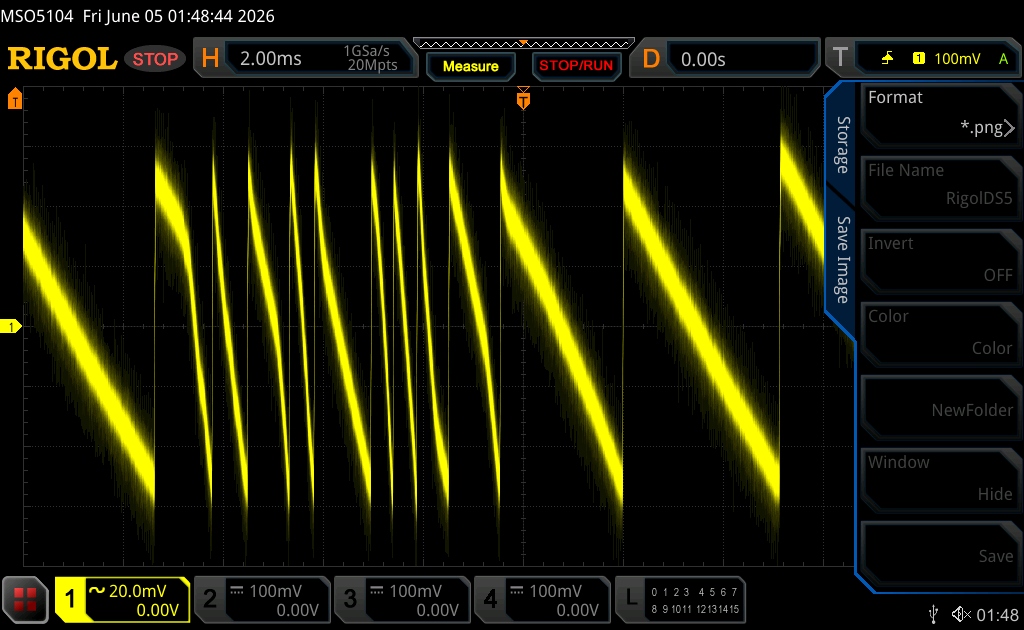
\includegraphics[width=0.85\textwidth]{figures/rail_ripple.png}
    \caption{Measured \SI{3.3}{\volt} rail ripple showing dynamic skip-mode behavior with non-constant switching frequency.}
    \label{fig:dc_dc_ripple_dynamic}
\end{figure}
    
\subsection{OLED Display Startup Issue}

During certain operating conditions, the OLED display failed to initialize correctly at board power-up. Specifically, the display remained off and did not enter its normal operating state. The issue was traced to an incorrect generation of the internal high-voltage rail required by the display driver.

The OLED module integrates an internal charge pump that generates the \SI{7.5}{\volt} supply required for display operation, using the external logic supply rail as its input. This supply is nominally specified in the range of \SIrange{3.3}{4.2}{\volt}. Because of the DC-DC buck controller regulation error, this supply rail was slightly degraded, measuring approximately \SI{3.26}{\volt}, and was further affected by significant introduced \SI{120}{\milli\volt} ripple (as described in the previous subsection). This combination of reduced DC level and superimposed ripple caused the SSD1306 charge pump to intermittently fail its start-up condition. In practice, the input voltage fell close to or below the internal start-up threshold of the charge pump control circuitry, preventing the generation of the required \SI{7.5}{\volt} internal supply. As a result, the display driver remained inactive and the OLED did not turn on. The issue was not observed when the system was powered from a clean \SI{3.3}{\volt} LDO-regulated supply. Under these conditions, the SSD1306 consistently succeeded in enabling the charge pump and correctly generating the internal high-voltage rail, resulting in reliable display initialization.

An additional dependency was observed on the system power-down state. When the board was powered after a sufficiently long off-time, allowing the discharge of the onboard capacitors, the initial power-up transient was sufficient to trigger correct charge pump start-up. However, during consecutive power cycles performed in quick succession, residual charge on the supply network reduced the effective startup transient amplitude. In these cases, the voltage step was insufficient to overcome the unknown internal start-up threshold of the charge pump, leading again to failure in generating the \SI{7.5}{\volt} rail and consequently preventing display activation.

\section{Possible Solutions and Future Improvements}

Since both observed issues are related to the quality and level of the \SI{3.3}{\volt} power rail, a single design modification can address them simultaneously. In particular, the system must satisfy two competing requirements: providing a clean, low-noise supply for the microcontroller and analog sensing circuitry, while also ensuring a sufficiently high input voltage for reliable startup of the OLED module internal charge pump.

To meet these constraints, the existing DC-DC buck converter is retained in order to preserve high overall efficiency during operation. However, its output voltage is adjusted slightly above the nominal \SI{3.3}{\volt} level, for example to \SI{3.5}{\volt} or \SI{3.6}{\volt}. This increase ensures that, even in the presence of ripple and transient voltage drops, the OLED driver input remains above the minimum start-up threshold required for correct charge pump operation, thereby improving initialization robustness.

A secondary low-dropout (LDO) regulator is then used to derive a clean and stable \SI{3.3}{\volt} rail from this intermediate voltage. Given the small voltage difference between \SI{3.5}{\volt}--\SI{3.6}{\volt} and \SI{3.3}{\volt}, the LDO operates with minimal power dissipation while effectively attenuating the switching ripple introduced by the buck converter. This configuration ensures a low-noise supply for sensitive analog and digital subsystems, including the MCU, the PAC1951 sensing circuitry, and the NTC temperature measurement network.

As a trade-off, the introduction of the LDO regulator introduces an additional power dissipation stage, leading to a reduction in overall system efficiency. Although the OLED display is not powered through the LDO, the regulator still supplies a portion of the system load which draw a few milliamperes under normal operation. The resulting voltage drop between the intermediate rail and the regulated \SI{3.3}{\volt} output leads to continuous power dissipation across the LDO. Nevertheless, this efficiency penalty is considered acceptable, as the affected currents are relatively low and the overall impact on the system power budget remains limited. In return, the proposed architecture significantly improves supply integrity, reduces ripple on sensitive analog circuitry, and increases the robustness of the OLED charge pump startup.

\begin{figure}[H]
\centering
\begin{tikzpicture}[
    node distance=1.2cm and 1.5cm,
    block/.style={draw, rounded corners, minimum width=2.8cm, minimum height=0.9cm, align=center},
    arrow/.style={->, thick}
]

% Nodes
\node[block] (vin) {Battery / Input Supply};

\node[block, below=of vin] (buck) {DC-DC Buck Converter\\(Vout = 3.5-3.6 V)};

\node[block, below left=of buck] (oled) {OLED Module\\(Charge Pump Input)};

\node[block, below right=of buck] (ldo) {LDO Regulator\\3.3 V Rail};

\node[block, below=of ldo] (v33) {MCU, \\PAC1951,\\ NTC};

% Connections (shortened arrows)
\draw[arrow, shorten >=2pt, shorten <=2pt] (vin) -- (buck);

\draw[arrow, shorten >=2pt, shorten <=2pt] (buck) -- (oled);

\draw[arrow, shorten >=2pt, shorten <=2pt] (buck) -- (ldo);

\draw[arrow, shorten >=2pt, shorten <=2pt] (ldo) -- (v33);

\end{tikzpicture}
\caption{Proposed power supply architecture with boosted buck output and post-regulation LDO for low-noise 3.3 V rail.}
\label{fig:power_supply_tree}
\end{figure}